\section{Priority Scheduling}
\subsection{Data Structures}
\paragraph{A1: (5 marks)}
Copy here the declaration of each new or changed `struct' or `struct' member, global or static variable, `typedef', or enumeration.  Identify the purpose of each in 25 words or less.

synch.h:\\
Added to struct lock :
\begin{verbatim}
    int priority;               /* Caches priority of threaads in lock. */
    struct list_elem elem;      /* Used in thread.c */
\end{verbatim}
Locks now cache the priority of the most important thread in their waiting list (this number is PRI\_MIN for empty waiting lists).\\ \\

thread.h:
\begin{verbatim}
/* Lists various structures that thread can be waiting on. */
enum blocker_type
  {
    NONE,      /* Thread is running or in ready list. */
    SEMA,      /* Thread is waiting on a semaphore. */
    LOCK,      /* Thread is waiting on a lock. */
    COND       /* Thread is waiting on a conditional. */
  };
\end{verbatim}

Added to struct thread:
\begin{verbatim}
    /* Added for priority sorting and donations. */
    struct list locks;                  /* Locks acquired by the thread. */
    void *blocker;                      /* Struct that blocks this thread.*/
    enum blocker_type type;             /* What is blocking the thread? */
\end{verbatim}
Threads now keep track of the locks they have acquired and the structure (if any) that they are waiting on.


\subsection{Algorithms}
\paragraph{A2: (10 marks)}
Explain the data structure used to track priority donation. Give a diagram that illustrates a nested donation in your structure.
\\
\\
Our implementation of priority donation does not rely on a single data structure. Instead, it is divided between struct lock and struct thread. Threads keep track of the locks they acquire, as well as the type of and pointer to the synch struct that they are waiting on, if applicable. Locks cache the priority of their most important waiting thread, avoiding unnecessary (and possibly recursive) calls into that thread to find out its priority.

In addition, the waiting lists for semaphores (by extension, locks) and condition variables order threads by priority, which makes it possible to track priority passively: finding the highest priority in a list of threads is simply a matter of looking at the head. The same is true of ready\_list: finding the next thread to run is done by popping its head.

When a thread attempts to acquire a lock that is held by another thread, the lock checks if its priority is higher than the cached priority. If it is, the newly blocked thread\'s priority is \"donated\" to the holder thread. This is done by reinserting the lock into the holder thread's list of acquired locks, ordered by descending donated priority. Again, since these locks are listed in order, finding the lock donating the highest priority is a simple matter of looking at the head of this list (and the thread's effective priority can be easily calculated by comparing this with its base priority).

If priority donation updates a blocked thread's priority, we may need to recursively propagate this new donated priority if the blocker is a lock. Firstly, the blocked thread notifies the structure it is waiting on to re-order its waiting list to reflect the change of priority.
In the case of a semaphore, the blocked thread whose priority was modified is simply reinserted into the list (condition variables reinsert the semaphore that blocks the thread in question).
In the case of a lock, the waiting list is reordered like it is for semaphores, and if the lock determines that the highest priority has changed, it notifies the thread that holds it to reorder its list of acquired locks. If this thread is also blocked, the recursion continues.
\\
\\
Much of the above is also covered by the below sequence of diagrams, which illustrates a nested priority donation:
\\
\\
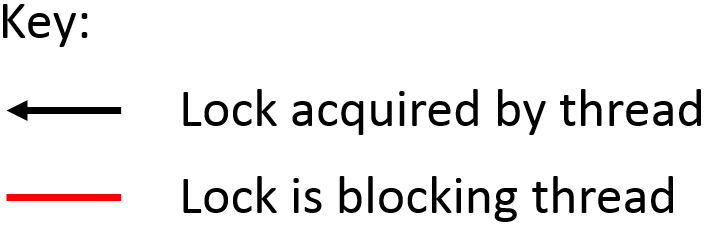
\includegraphics[scale=0.35]{Key}

\newpage
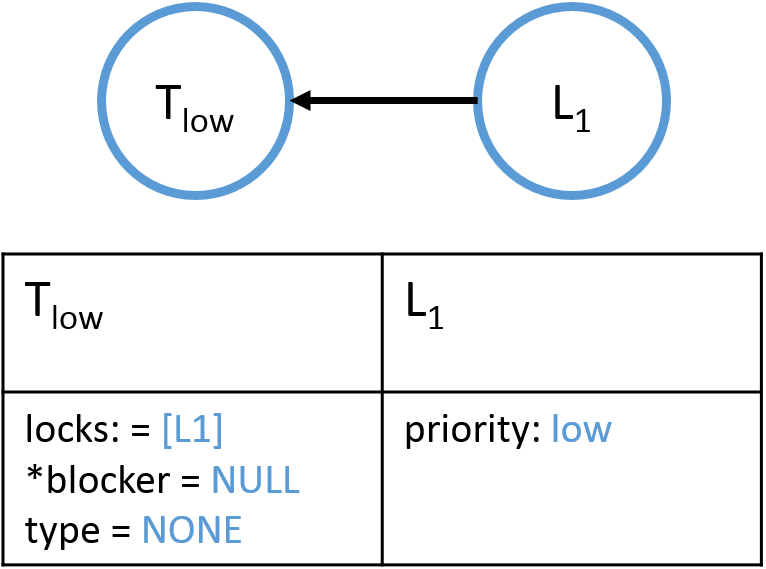
\includegraphics[scale=0.45]{A1}
\\
\\
A low priority thread has acquired L1.
\\
\\
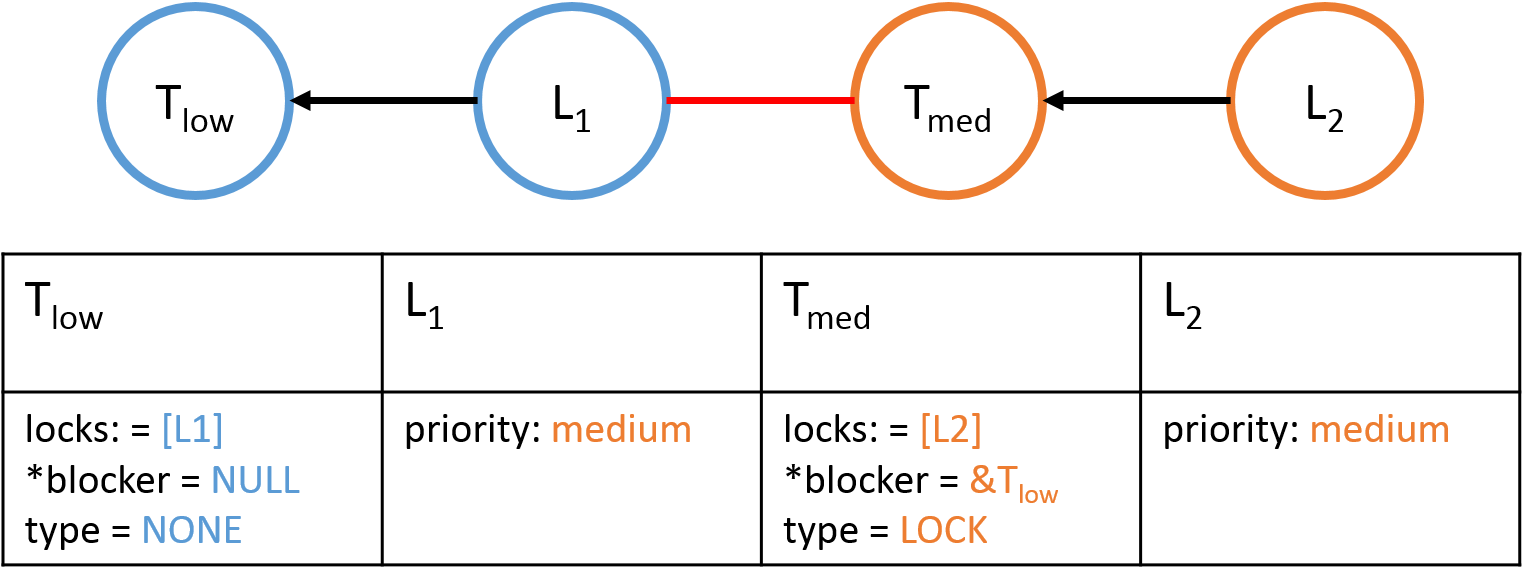
\includegraphics[scale=0.45]{A2}
\\
\\
A medium priority thread then acquires L2 before attempting to acquire L1. Because L1 has already been acquired by TLow, TMed is inserted into L1's waiters list, thus increasing the priority of L1 to its own. Because the L1's priority has changed, we must reorder TLow's locks list, thereby donating TMed's priority to TLow. TMed then checks whether TLow is being blocked, and since it is not, nothing further happens.
\\
\\
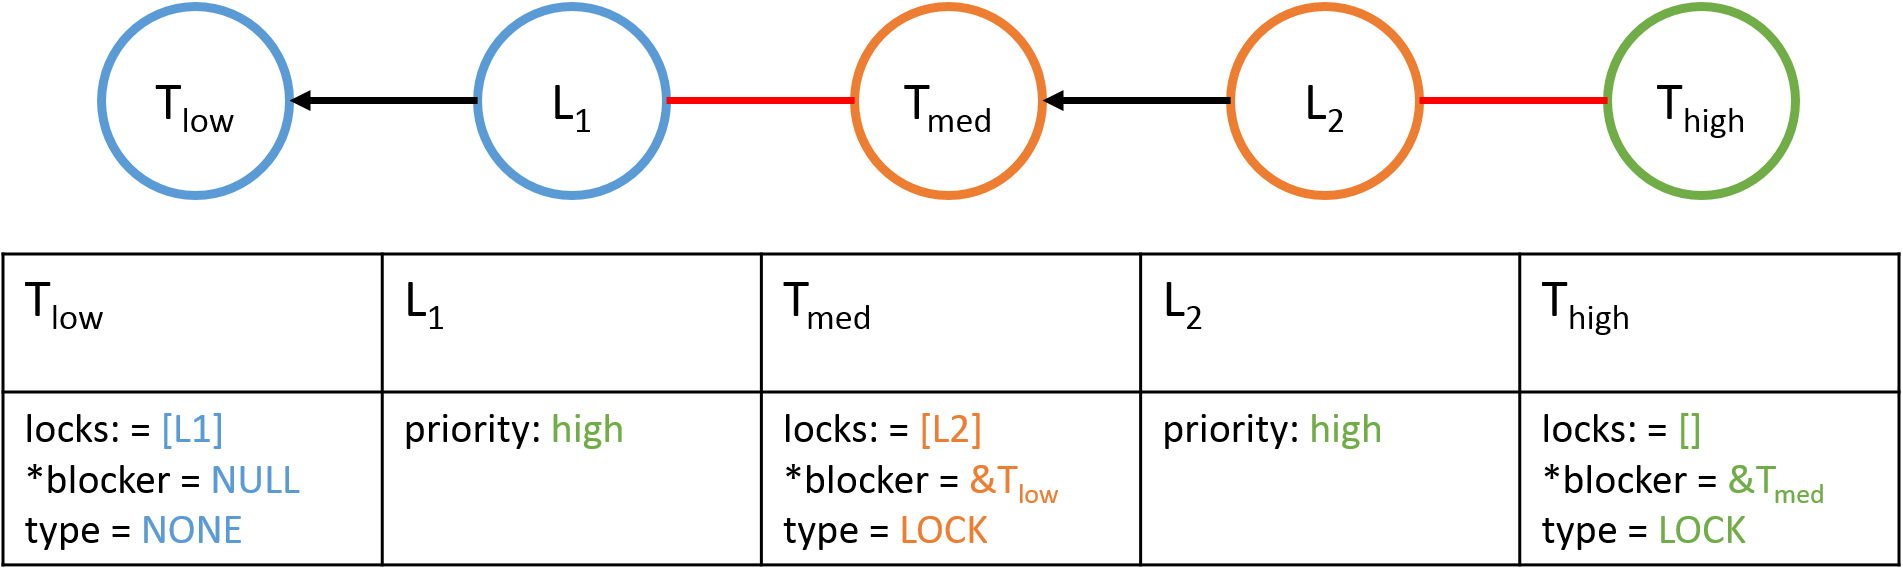
\includegraphics[scale=0.45]{A3}
\\
\\
A high priority thread now attempts to acquire L2. Because L2 is already held by TMed, THigh is inserted into L2's waiters list, L2's priority is increased and high priority is donated to TMed. Now, since TMed is being blocked by another lock, we must recurse. L1's list of waiters is reordered, and this causes its priority to also increase to high (since TMed now has high priority). This in turn triggers TLow's locks list to be reordered, finally donating high priority to TLow.
\\
\\
\paragraph{A3: (5 marks)}
How do you ensure that the highest priority thread waiting for a lock, semaphore, or condition variable wakes up first?
\\
\\
Our implementation guarantees that the lists of waiting threads inside semaphores (by extension, locks) and condition variables are sorted in order of decreasing effective priority.

We maintain this guarantee by inserting threads into the waiting list with list\_insert\_ordered(), which uses an auxiliary function to compare thread priorities.
When a thread's effective priority changes through priority donation, if this thread is waiting in a list, we reinsert the thread into the list, thus maintaining its order. If it waiting on a lock, if the highest priority of the lock's waiting list is changed, this change is propagated to the holder of the lock.

When a semaphore, lock or condition variable wakes up a thread, it simply pops the front of the waiting queue, which we know is ordered. Hence when a thread is released from the waiters list, it is guaranteed to be (one of) the thread(s) with highest priority.

\paragraph{A4: (5 marks)}
Describe the sequence of events when a call to lock\_acquire() causes a priority donation.  How is nested donation handled?
\\
\\
In order for priority donation to happen, a low priority thread (say thread A) has to first acquire the lock. This points the lock's holder to thread A, and inserts the lock into thread A's list of acquired locks.

Then when thread B calls lock\_acquire on the same lock, it is blocked. This first sets the blocker pointer at the lock and blocker\_type to LOCK. It then updates the lock's cached priority through lock\_try\_increase\_priority(), which also returns whether the priority increased or not.

In this case, we shall assume that thread B has a higher priority than any thread in the lock's waiters list (or that the list is empty). Therefore, the lock's priority will increase and lock\_try\_increase\_priority() will return true. We now need to inform the lock holder's thread (i.e. thread A) that the lock is now donating a higher priority, and thus it must reorder its list of locks (by calling thread\_notify\_blocker()). This reordering indirectly causes thread B to donate its priority to thread A, since A's list of locks are sorted in descending priority, and its donated priority is found by simply looking at this list's head.

If thread A itself is blocked, then we will need to inform its blocker. Since we are considering a nested donation scenario, this blocker will be another lock which we will need to recurse into. Because thread A has just had its priority changed and it is waiting for this lock, we will have to reorder the lock's waiters list by calling lock\_reinsert\_thread(). We then need to check if the overall priority of the lock has changed, and inform the lock's holder whether this is the case. If the holder is also blocked, the recursion will continue.

\paragraph{A5: (5 marks)}
Describe the sequence of events when lock\_release() is called on a lock that a higher-priority thread is waiting for.
\\
\\
We shall assume that the higher priority priority thread (say thread B) is at the head of the lock\'s waiters list, and is donating its priority to the thread holding the lock (say thread A).

Firstly, thread A calls lock\_release(). This resets the lock's holder to NULL and removes the lock from thread A\'s list of acquired locks (interrupts are also disabled here to synchronise access to this list as it may be accessed in an interrupt handler).

The lock's cached priority is then recalculated (by getting the priority of the 2nd waiting thread, or returning PRI\_MIN if it doesn't exist) before sema\_up() removes the 1st waiting thread (say thread B) from the waiters list and calls thread\_unblock() on it.

This function resets thread B\'s blocker pointer and enum, sets its status to THREAD\_READY and inserts it into the ready list.

In this case, thread B\'s effective priority is now higher than the currently running thread A (as removing the lock from thread A\'s list of locks also removes any priority which it donated), so it gets must get placed at the head of the ready\_list (since thread A previously held the highest priority in ready\_list before it lost its donated priority and awakened thread B). A call to thread\_yield() is also triggered, causing thread B to pre-empt thread A and begin running.

\subsection{Synchronisation}
\paragraph{A6: (5 marks)}
Describe a potential race in thread\_set\_priority() and explain how your implementation avoids it.  Can you use a lock to avoid this race?
\\
\\
In priority donation, thread\_set\_priority() is only used by the current thread to alter its own base priority (that is, its variant, thread\_set\_priority\_of() is never called).

As in priority scheduling, the thread with the highest priority must be running at all times, the purpose of thread\_set\_priority() is two-fold: it sets the base priority of the thread and if the effective priority of the thread is now lower than the priority of a thread on the ready list, it calls thread\_yield().

The race condition may occur during this access to the ready list: for instance, another thread of the same priority as the current thread may be scheduled at the head of the ready list (for instance, after being woken from sleep by timer\_interrupt), but the current thread already fetched the head of the list, it would not yield, even though it should.

Hence, access to the ready list need to be synchronised to prevent this sort of error. As the ready list is shared between the threads and the interrupt handler, the only way to do so is to disable interrupts, as locks cannot be acquired in the context of an interrupt handler.


\subsection{Rationale}
\paragraph{A7: (5 marks)}
Why did you choose this design?  In what ways is it superior to another design you considered?
\\
\\
Throughout the development of the implementation of priority donations (and of the priority scheduling that underlies both this task and the mlfqs system) we have considered several systems, most of them building on our previous design decisions.

In developing priority scheduling, we decided to use priority queues for the waiting lists in semaphores and condition variables, and the ready list, as this trivialised finding the thread with the highest priority.

As priority donation is closely related to locks and lock ownership, we decided that it would be simplest to have threads to keep track of the locks that they are currently holding. This list is ordered by priority of the most important thread in each lock's waiting list.

Keeping in line with these decisions, we had to ensure that priority donations kept these lists ordered, which lead to the creation of methods like thread_reinsert_lock, which is called when a lock's priority is changed, and lock_reinsert_thread(), which is called when a thread's priority is changed.

In order to speed up the reinsertion operation, locks cache the highest priority of the threads in their waiting list, which is updated when a thread is added to or removed from it. This meant that thread_get_priority_of() was no longer a recursive call that walked down the chain of acquired locks and threads waiting on those locks.

Finally, the reinsert operations were made mutually recursive by making threads keep track of the lock that they are waiting on, allowing priority donation to propagate up the lock ownership chain.

The resulting system was fairly simple and flexible, which made it easy to integrate condition variables, as well as mesh with the mlfqs system.


During development, we briefly considered using unordered lists and list_max to find the highest priority thread when it was needed, as this would largely simplify list updates (the lists would not need to be changed when the priority of their elements changes) and require less interrupt disabling.

This idea cropped up multiple times, however it was rejected as it made it difficult to update lock priorities in large lock-list-lock chains and if caching was dropped completely, getting a thread's priority would have a worst case running time of O(n-1), where n is the number of threads, as the call would need to check the priority of every thread that is waiting on the thread whose priority we are evaluating.

Moreover, the worst case running time of list_max is identical to its best case running time, which is O(n), where n is the number of elements in the list.
Of course, the worst case of list_insert_ordered (used in both the reinsert methods and the methods that add threads to lists) is also O(n), however its best case is constant.
We considered that list updates, which are more efficient for unordered lists, do not take place often enough to offset the cost of retrieving the most important element from a list every time an element needs to be removed or the inefficiency of thread_get_priority.

We also considered different types of lists for tracking priority donations (such as keeping track of donating threads directly, or keeping track of the priority values, but not the structures that donate them), however, keeping a list of locks turned out to be the simplest to implement among them, as adding and removing priorities could simply be done through lock_acquire and lock_release.

Another concern we had during development was synchronising list access 

Talk about:
	caching priorities in locks
	using priority queues for the list of locks
  removing/reinserting element vs calling resort() on list <-- more efficient?
	disabling interrupts being necessary? (We didn't come up with a viable solution that could avoid these though, besides a lock for a list of locks which could block the scheduler)
